%---------------------------------------------------------
%	Packages and doc config
%---------------------------------------------------------

\documentclass{report}

% \setlength\parindent{0pt} % Removes all indentation from paragraphs

\usepackage[table]{xcolor}% http://ctan.org/pkg/xcolor

\usepackage[english]{babel}

\usepackage[english]{babel}
\usepackage[utf8]{inputenc}
\usepackage[margin=3cm]{geometry}
\usepackage{graphicx}
\usepackage{todonotes}
\usepackage{float}
\usepackage{amsmath}
\usepackage{subcaption}
\usepackage{listings}
\usepackage{color}
\usepackage{wrapfig}
\usepackage{titling}
\usepackage{multicol}
\usepackage{amsmath}


\renewcommand{\lstlistingname}{Code Snippet}

\lstdefinestyle{customc}{
  belowcaptionskip=1\baselineskip,
  breaklines=true,
  language=C,
  showstringspaces=false,
  basicstyle=\ttfamily,
  keywordstyle=\bfseries\color{green!40!black},
  commentstyle=\itshape\color{purple!40!black},
  identifierstyle=\color{blue},
  stringstyle=\color{orange},
}

\lstdefinestyle{customv}{
  belowcaptionskip=1\baselineskip,
  breaklines=true,
  showstringspaces=false,
  basicstyle=\footnotesize\ttfamily,
}

%\usepackage{times} % Uncomment to use the Times New Roman font

%---------------------------------------------------------
%	Document
%---------------------------------------------------------

\title{CM30225 Parallel Computing\\Shared Memory} % Title
\author{Rowan Walshe} % Author name

\date{\today} % Date for the report

\begin{document}

\maketitle % Insert the title, author and date
\pagebreak

\chapter{Code}
\section{Introduction}
While working on this coursework, I tested a number of different solutions for parallelising the problem. In this section I will discuss these different approaches along with the advantages and disadvantages of each.

\section{Sequential Version}
For my sequential version of my program I used one of the programs that I created for the first part of this coursework. The main loop for this program can be seen  below in Code listing 1.1. The program moves through the 2D array from the top left down to the bottom right. At each point it the array it temporally stores the value at the point, then calculates the new value based on the average of the surrounding four values. It then checks to see if the absolute difference between the new and old value is greater than the given precision. If the value at any point changes more than the given precision, then at the end of this iteration of averaging values, it must complete at least one more iteration. By checking if the endFlag is still true before calculating the absolute difference, it reduces the number of times this difference needs to be calculated, reducing overall runtime. This is illustrated in Code Snippet 1.1.
\begin{lstlisting}[style=customc,caption=Version 1 Sequential Main Loop]
    while(1) {
        endFlag = true;
        iterations++;
        for(i=1; i<sizeOfPlane-1; i++) {
            for(j=1; j<sizeOfPlane-1; j++) {
                pVal = plane[i][j];
                plane[i][j] = (plane[i-1][j] + plane[i+1][j]
                    + plane[i][j-1] + plane[i][j+1])/4;
                if(endFlag && tolerance < fabs(plane[i][j]-pVal))
                    endFlag = false;
            }
        }
        if(endFlag)
            return iterations;
    }
\end{lstlisting}
While working on the shared memory version of this coursework, I found that by accessing data in the array using a checkerboard pattern, I was able to guarantee the result of the program would always be the same, while also reduce runtime due to a lower cache miss rate. However for a distributed memory program, accessing data in this pattern had little to no effect on the run time, as any benefit was removed due to the increased overhead required for the extra MPI calls. Therefore, I decided to use this version instead of the checkerboard one for all my testing.
\section{MPI Version}
\subsection{Relexation Algorithm}
\begin{wrapfigure}{r}{0.35\textwidth}
\vspace{-30pt}
\includegraphics[width=0.35\textwidth]{grid}
\caption{Row Division}
\label{fig:subim1}
\end{wrapfigure}

I am using a similar method to the one I used in the shared memory coursework, in order to split the problem between MPI processes. Each MPI process is assigned a certain number of rows to work on, based on its world rank. In the example shown in Figure 1.1, an 11x11 array is split up between three MPI processes, with each process being assigned three rows. Each process frees memory for an array that contains two more rows than it is going to run the relaxation algorithm on. This is because each MPI process needs access to the values of the row above and below the first and last row that it will be doing work on. On top of this, by reducing the amount of data that each process has to keep in memory, as well as the amount of memory needed per node, it is easier to scale to run larger problem sizes as you are not limited by the amount of memory that you could reasonably fit in a shared memory system. The code for the computation that each MPI process does on its part of the array can be seen bellow in Code Snippet 1.2. This code should be recognisable from the sequential program, with the only difference being the number of rows that work is done on.

\begin{lstlisting}[style=customc,caption=MPI Relaxation Computation]
    for(i=1; i<recBot; i++) {
        for(j=1; j<sizeOfPlane-1; j++) {
            pVal = plane[i][j];
            plane[i][j] = (plane[i-1][j] + plane[i+1][j] + plane[i][j-1] + plane[i][j+1])/4;
            if(endFlag && tolerance < fabs(plane[i][j]-pVal))
                endFlag = false;
        }
    }
\end{lstlisting}

\subsection{MPI Communication}
After each iteration, every MPI process sends the top and bottom row that it worked on to the corresponding MPI processes, and then receives updated data into the first and last row of its 2D array. The one exception to this is the MPI process with world rank zero, which only sends and receives data to and from the bottom of its array, and the last MPI process which only sends and receives data to and from the top of its array.

\newpage

\begin{figure}[h]
%n\vspace{100pt}
\includegraphics[width=1\linewidth]{mpi-com} 
\caption{MPI Communication Pattern}
\label{fig:subim2}
\end{figure}

\begin{lstlisting}[style=customc,caption=MPI Communication]
    // Send and Recieve data depending on the world_rank
    if(world_rank==0) {
        // Only send data down to process with world_rank 1
        MPI_Isend(&plane[sendBot][1], sizeOfInner, MPI_DOUBLE, 1, 0, MPI_COMM_WORLD, &myRequest1);
        MPI_Recv(&plane[recBot][1], sizeOfInner, MPI_DOUBLE, 1, 0, MPI_COMM_WORLD, MPI_STATUS_IGNORE);
    } else if(world_rank==world_size-1) {
        // Only send and recive/data to the process above i.e. world_rank-1
        MPI_Isend(&plane[1][1], sizeOfInner, MPI_DOUBLE, world_rank-1, 0, MPI_COMM_WORLD, &myRequest1);
        MPI_Recv(&plane[0][1], sizeOfInner, MPI_DOUBLE, world_rank-1, 0, MPI_COMM_WORLD, MPI_STATUS_IGNORE);
    } else {
        // Send new data up
        MPI_Isend(&plane[1][1], sizeOfInner, MPI_DOUBLE, world_rank-1, 0, MPI_COMM_WORLD, &myRequest1);
        // Send new data down 
        MPI_Isend(&plane[sendBot][1], sizeOfInner, MPI_DOUBLE, world_rank+1, 0, MPI_COMM_WORLD, &myRequest2);
        // Receive new data from above
        MPI_Recv(&plane[0][1], sizeOfInner, MPI_DOUBLE, world_rank-1, 0, MPI_COMM_WORLD, MPI_STATUS_IGNORE);
        // Receive new data from below
        MPI_Recv(&plane[recBot][1], sizeOfInner, MPI_DOUBLE, world_rank+1, 0, MPI_COMM_WORLD, MPI_STATUS_IGNORE);
    }
\end{lstlisting}

I'm using \lstinline[style=customc]|MPI_Isend()| instead of \lstinline[style=customc]|MPI_Send()| as I hit a buffer size limit on balena when attempting to send rows over 2002 long, causing the program to hang. This is a non blocking send which means that each MPI process moves on to attempting to receive data, no matter weather or not it has actually finished sending data yet. This could cause issues, however as I use the blocking version of receive, followed by an MPI call to bring together the endFlag from each MPI process, each process never attempts to start a new iteration until all new data has finished being sent and received. To bring together the endFlag from each process I use another MPI function, \lstinline[style=customc]|MPI_Allreduce()|, which can be seen below in Code Snippet 1.4.

\begin{lstlisting}[style=customc,caption=MPI Communication]
    MPI_Allreduce(MPI_IN_PLACE, &endFlag, 1, MPI_INT, MPI_LAND, MPI_COMM_WORLD);
\end{lstlisting}

The MPI\_op MPI\_LAND makes the Allreduce perform a logical and between the endFlag of all of the MPI processes. Therefore if any one of the endFlags is false, then all of them become false, and do another iteration.

\subsection{Result Output}
Initially when the program had finished, in order to output the full plane, I was initially gathering all the data on to the MPI process with world rank 0, from which it would become trivial to either print the result to stdout, or write it to a file. In order to call an MPI\_Gatherv function, the root node had to calculate how many bytes it would be receiving from each MPI process, as well as the offset from the start of the receiving buffer it was to write the data to. The code for this can bee seen below in Code Snippet 1.5

\begin{lstlisting}[style=customc,caption=How to Gather Data onto One MPI Process]
    int sizeOfInner = sizeOfPlane-2;
    int rowsPerThreadS = sizeOfInner/world_size+1;
    int rowsPerThreadE = sizeOfInner/world_size;
    int remainingRows = sizeOfInner - world_size * rowsPerThreadE;

    int tempNumRows;
    int* recvcounts = malloc((unsigned int)world_size * sizeof(int)); 
    int* displs = malloc((unsigned int)world_size * sizeof(int));

    // Calculate recvcounts and displs 
    for(int i=0; i<world_size; i++) {

        if(i < remainingRows) {
            tempNumRows = rowsPerThreadS;
        } else {
            tempNumRows = rowsPerThreadE;
        }

        recvcounts[i] = tempNumRows * sizeOfPlane;
        if(i < remainingRows) {
            displs[i] = (i * rowsPerThreadS) * sizeOfPlane;
        } else {
            displs[i] = (i * rowsPerThreadE + remainingRows) * sizeOfPlane;
        }
    }
    
    MPI_Gatherv(&subPlane[1][0], (numRows-2)*sizeOfPlane, MPI_DOUBLE, &plane[1][0], recvcounts, displs, MPI_DOUBLE, 0, MPI_COMM_WORLD);
\end{lstlisting}
However in my final version I wrote some code in order to be able to output the results to a file without having to gather all of the data in to a single process. While my implementation, which can be seen below in Code snippet 1.6, uses the standard C library for file input output, I also could have used a number of MPI file writing functions such as \lstinline[style=customc]|MPI_File_write_at()| in order to have all of the MPI processes to write to the file at the same time, without having to use a barrier.

\begin{lstlisting}[style=customc,caption=Write Results to File]
    FILE* file;
    char* file_name;
    // Create the file name, so it is easy to see at a glance the world_size and problem size that the results came from
    asprintf(&file_name, "%d-%d.result", world_size, sizeOfPlane);

    for(int i=0; i<world_size; i++) {
        // If it is this processes turn, write out to the file
        if (i == world_rank) {
            // If this is world_rank 0 then create a new file, otherwise append to the existing file
            file = fopen(file_name, world_rank == 0 ? "w" : "a");
            
            // Unless this is the first or last MPI process, do not write out the first or last line of the array
            int startingRow = 1;
            int endingRow = numRows - 1;
            // If this is the first or last MPI process, then also write out the first or last line of the array respecively
            if(world_rank == 0) {
                startingRow = 0;
            } else if(world_rank == world_size-1) {
                endingRow = numRows;
            }
            // Write out data from the array
            for(int j=startingRow; j<endingRow; j++) {
                for(int k=0; k<sizeOfPlane; k++)
                    fprintf(file, "%f, ", subPlane[j][k]);
                fprintf(file, "\n");
            }
            fclose(file);
        }
        MPI_Barrier(MPI_COMM_WORLD);
    }
    // Additional information about how the program ran
    if(!world_rank) {
        file = fopen(file_name, "a");
        fprintf(file, "\nThreads: %d\n",world_size);
        fprintf(file, "Size of Pane: %d\n", sizeOfPlane);
        fprintf(file, "Iterations: %lu\n", iterations);
        fprintf(file, "Time: %Lfs\n", toSeconds(start, end));
        fclose(file);
    }
\end{lstlisting}

\chapter{Correctness Testing}
I was able to confirm that for small test sizes my final program was correct by manually calculating the result by hand and comparing my result with that of my program. Due to how I am traversing data in the 2D array, I do not have any race conditions that could affect the result outputted by my program. This means that if the result is correct for the sequential algorithm, then it will also be correct for the parallel algorithm.
While I was not able to print out the result of every single run, as I would have run out of storage space, and some of the programs would have run out of time, I did compare a number of results. For all of the tests that I did print results from, the solution was identical for all of them. For each test I also printed out the number of iterations that the program took to reach a solution, so that if there was an error that only happened occupationally, but affected the result, it would have been much easier to spot.
\chapter{Scalability Testing}
To measure the performance of my parallel algorithms, I gathered a large range of results from balena, using various thread counts and problem sizes. I will be using a number of common metrics including speedup, efficiency, and the Karp-Flatt Metric to discuss the performance and scalability of my MPI program.\newline

Speedup on P processors is equal to the time to run the sequential algorithm divided by the time to run the parallel algorithm on p processors. This assumes that the problem size is constant.

$$Speedup\ _p=\frac{Sequential\ Time}{Parrallel\ Time\ _p}$$\newline1

Efficiency is equal to the amount of speedup per processor. It is a measure of how efficiently my parallel algorithm is using the extra processors.

$$Efficiency\ _p=\frac{S_p}{p}=\frac{Sequential\ Time}{p\times Parrallel\ Time\ _p}$$\newline

The Karp-Flatt metric can be used to effectively measure the sequential portion of parallel programs. Generally it is between zero and one, though may be more than one if there is slowdown, or less than zero if there is superlinear speedup.\newline

$$e=\frac{\frac{1}{S_p}-\frac{1}{p}}{1-\frac{1}{p}}$$\newline

Overhead is required to calculate isoefficiency. It effectively tells us how much extra time was added in overheads while parallelising the sequential algorithm. A smaller overhead also means that the parallel algorithm is work efficient.\newline

$$T_o=pT_p - T_s$$\newline

Isoefficiency allows me to measure how scalable my parallel algorithm is. It is generally between zero and one. The closer isoefficiency is to one, the better it scales.\newline

$$E=\frac{1}{1+\frac{T_o}{T_s}}$$\newline
\section{Time to Run}
To test the scalability of my different algorithms, I measure the time that it took to complete the start up and relaxation part of the program, for various problem sizes and MPI process counts using a precision of 0.0001. Instead of using the time given by the output from balena, I used \lstinline[style=customc]|clock_gettime()|\lstinline[style=customc]|| which can be found in the standard C time library. This allowed me to measure the runtime more precisely, to within 0.000001 seconds. It also allowed me to removed overheads from the timing that could be introduced while the OS starts and cleans up after the program. In practice this overhead becomes insignificant as the problem size increases, as it is something that only has to be done once per run. For version one I ran all my tests three times and calculated the average.

As you can see in Figure 3.1, there is a large reduction in runtime from V1 to V2. which allowed me to test much larger problem sizes. As I explained in section 1.3,  I believe the main reason for this is due to more efficient memory accessing. As you can see in Figure 3.1b and 3.2 there is again a slight decrease in time to run between V2 and V3.

\begin{figure}[h]
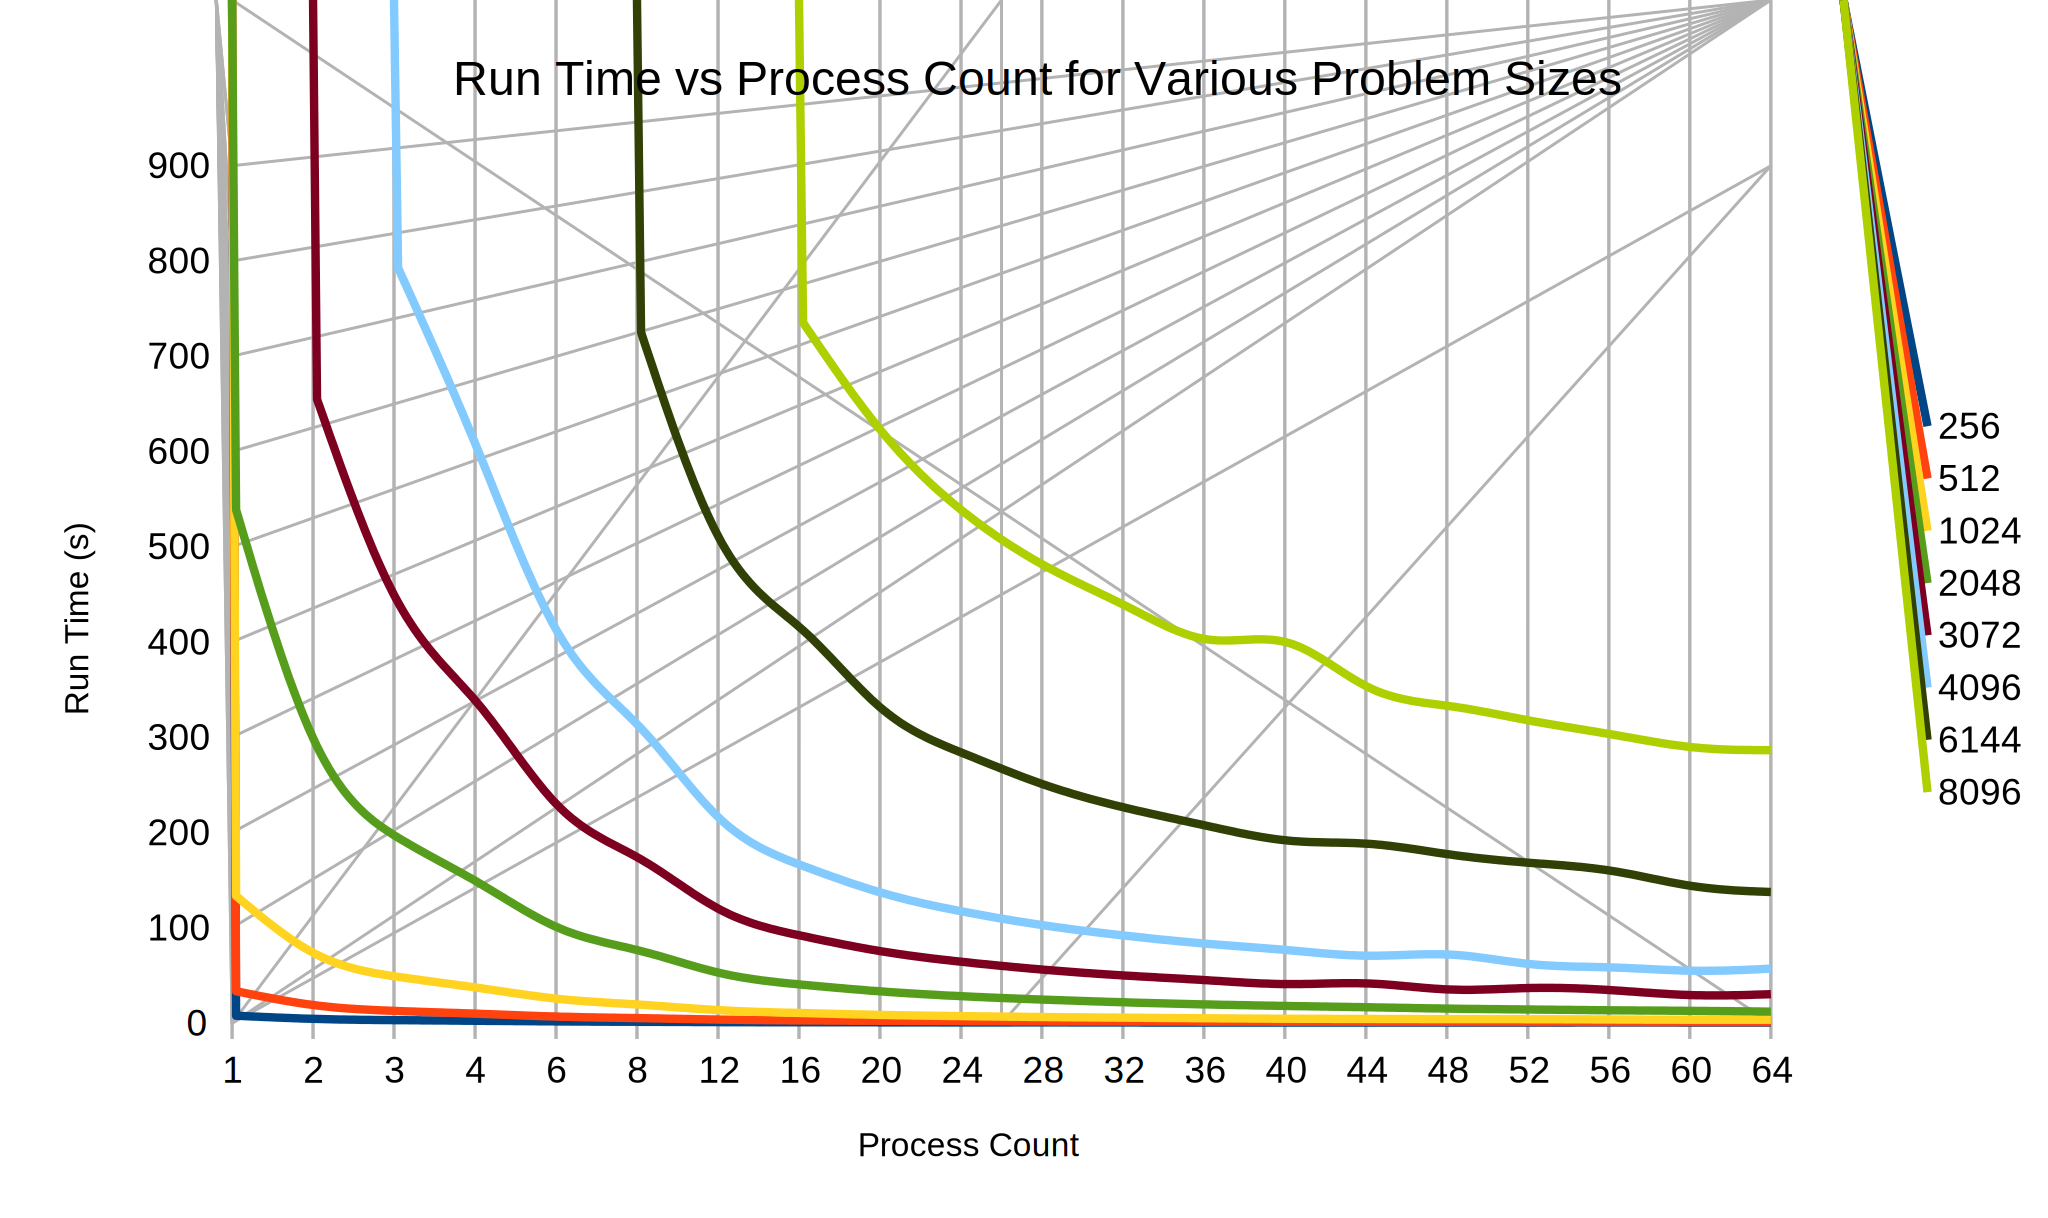
\includegraphics[width=1\textwidth]{Runtime}
\caption{Version 3 Timings}
\label{fig:subim3}
\end{figure}
\pagebreak
\section{Speedup}
Using the timing results that I gathered, I was able to calculate speedup for different values of p, at different problem sizes. As you can see in Figures 3.3 and 3.4, all of the parallel algorithms start off slower than than the sequentail, however by array size 250x250, all of them have speedup greater than one and so are finishing faster than their respective sequential algorithm. With some of the smaller processor counts you can see the speedup starts to level off. This is because of the Amdahl's law, which says that:
\begin{quote}
"Every program has a natural limit on the maximum speedup it can attain, regardless of the number of processors used"
\end{quote}
Unfortunately as there is a time limit for how long a program can run on balena for, we are unable to see where some of the larger threads counts speedup's level off. However as Gustafson's Law says, as the problem sizes get bigger, the sequential part effectively becomes smaller. Therefore I expect that if I was to be able to test larger problem sizes, the larger thread counts would continue to speedup.
\\\\
One oddity with my results is that for the problem sizes I was able to test, allowing the program to use 14 threads and even sometimes 12 threads, often outperforms the program that was allowed to use 16 threads. Initially I thought that I had made a mistake and was spawning one too many threads, however some simple testing by having each thread print out their thread ID, it was easy to show that this was not the case. It may be that if I was to continue to increase the problem size, 16 threads would eventually catch up and overtake them, however I was unable to test this hypotheses. 
\\\\
Finally, in a few cases the program actually gets superlinear speedup, for example for two, four and six threads of my final. This can bee seen in Figure 3.4 where the speedup lines go slightly above what you would expect their max speedup to be. There could be a few reasons for this, including that the sequential and parallel algorithms are fundamentally different, data is being more efficiently loaded into memory or there are slight variations in the time to run, that happens to cause superlinear speedup in some cases. I am pretty confident that both my sequential and parallel algorithms are so similar that this could not be the cause. While I tested the programs with cachegrind, the results did not show any noticable difference between how data was being pre-fetched for the single and parallel algorithms. However, due to how cachegrind works with multi-threaded programs, the results may not be as accurate compared to a single threaded program. Therefore I am unable to rule out how data is being pre-fetched as a reason for the slight superlinearity. On top of this, while running retests on Version 1, I noticed that even for the single threaded algorithm, there was slight differences in the time it took to run each time, which could also account for the small ammount of superlinear behaviour. Finally, as this superlinear behaviour is most prominent in my third version, there could be some intrinsic behaviour of AVX such as a warmup time that I do not know about and so have not taken into account.
\begin{figure}[h]
\begin{subfigure}{0.5\textwidth}
\includegraphics[width=1\linewidth, height=5cm]{V1-Speedup} 
\caption{Version 1 Timings}
\label{fig:subim4}
\end{subfigure}
\begin{subfigure}{0.5\textwidth}
\includegraphics[width=1\linewidth, height=5cm]{V2-Speedup} 
\caption{Version 2 Timings}
\label{fig:subim5}
\end{subfigure}
\caption{Version 1 and 2 Timings}
\end{figure}
\begin{figure}[h]
\includegraphics[width=1\textwidth]{V3-Speedup}
\caption{Version 3 Timings}
\label{fig:subim6}
\end{figure}

\section{Efficiency}
As stated earlier, efficiency is a measure of how efficiently my parallel algorithm is using the extra processors. For example, if a program has an efficiency of 0.5 for a given problem size an number of processors, then half of the time that the processors could be doing work, is lost to overheads. These graphs show that my algorithms scale pretty as efficiency increases as the problem size does. Another way thinking about this, is that with larger problem sizes, the efficiency decreases slower as the core count increases . This follows the reasoning of Gustafson's law. One thing to note, is that for some problem sizes and processor counts, V3 has lower efficiency than V1. However as V3 is so much faster than V1, I don't think this is much of an issue. Finally, these graphs more easily show the superlinear behaviour that was discussed in section 3.2, 1as efficiency can be seen going above 1.
\begin{figure}[h]
\begin{subfigure}{0.5\textwidth}
\includegraphics[width=1\linewidth, height=5cm]{V1-Efficiency} 
\caption{Version 1 Efficiency}
\label{fig:subim4}
\end{subfigure}
\begin{subfigure}{0.5\textwidth}
\includegraphics[width=1\linewidth, height=5cm]{V2-Efficiency} 
\caption{Version 2 Efficiency}
\label{fig:subim5}
\end{subfigure}
\caption{Version 1 and 2 Efficiency}
\end{figure}
\begin{figure}[h]
\includegraphics[width=1\textwidth]{V3-Efficiency}
\caption{Version 3 Efficiency}
\label{fig:subim6}
\end{figure}

\section{Karp-Flatt Metric}
Figures 3.7 and 3.8 show the Karp-Flatt metric of my algorithms at various array sizes. As the problem size increases, the Karp-Flatt metric decreases. This is consistent with Gustafson's law, which says that as the problem size increases, the effective sequential part of an algorithm decreases. In some of the tests, the Karp-Flatt metric is more than one as 
\begin{figure}[h]
\begin{subfigure}{0.5\textwidth}
\includegraphics[width=1\linewidth, height=5cm]{V1-Karp-Flatt} 
\caption{Version 1 Karp-Flatt}
\label{fig:subim4}
\end{subfigure}
\begin{subfigure}{0.5\textwidth}
\includegraphics[width=1\linewidth, height=5cm]{V2-Karp-Flatt} 
\caption{Version 2 Karp-Flatt}
\label{fig:subim5}
\end{subfigure}
\caption{Version 1 and 2 Karp-Flatt}
\end{figure}
\begin{figure}[h]
\includegraphics[width=1\textwidth]{V3-Karp-Flatt}
\caption{Version 3 Karp-Flatt}
\label{fig:subim6}
\end{figure}

\chapter{Conclusion}
My current solution scales well with core count and problem size, with the max recorded speedup being around 12. My results also show that the efficiency of my solution drops as expected, as the thread count increases. The lowest Karp-Flatt value that I messured was around 0.011. Using this value in conjunction with Amdahl's law, I can predict a max speedup of my algorithm on an array size 1600 will be around 90.
\end{document}